\documentclass{standalone}
\usepackage{tikz}
\usetikzlibrary{patterns, positioning}


\begin{document}
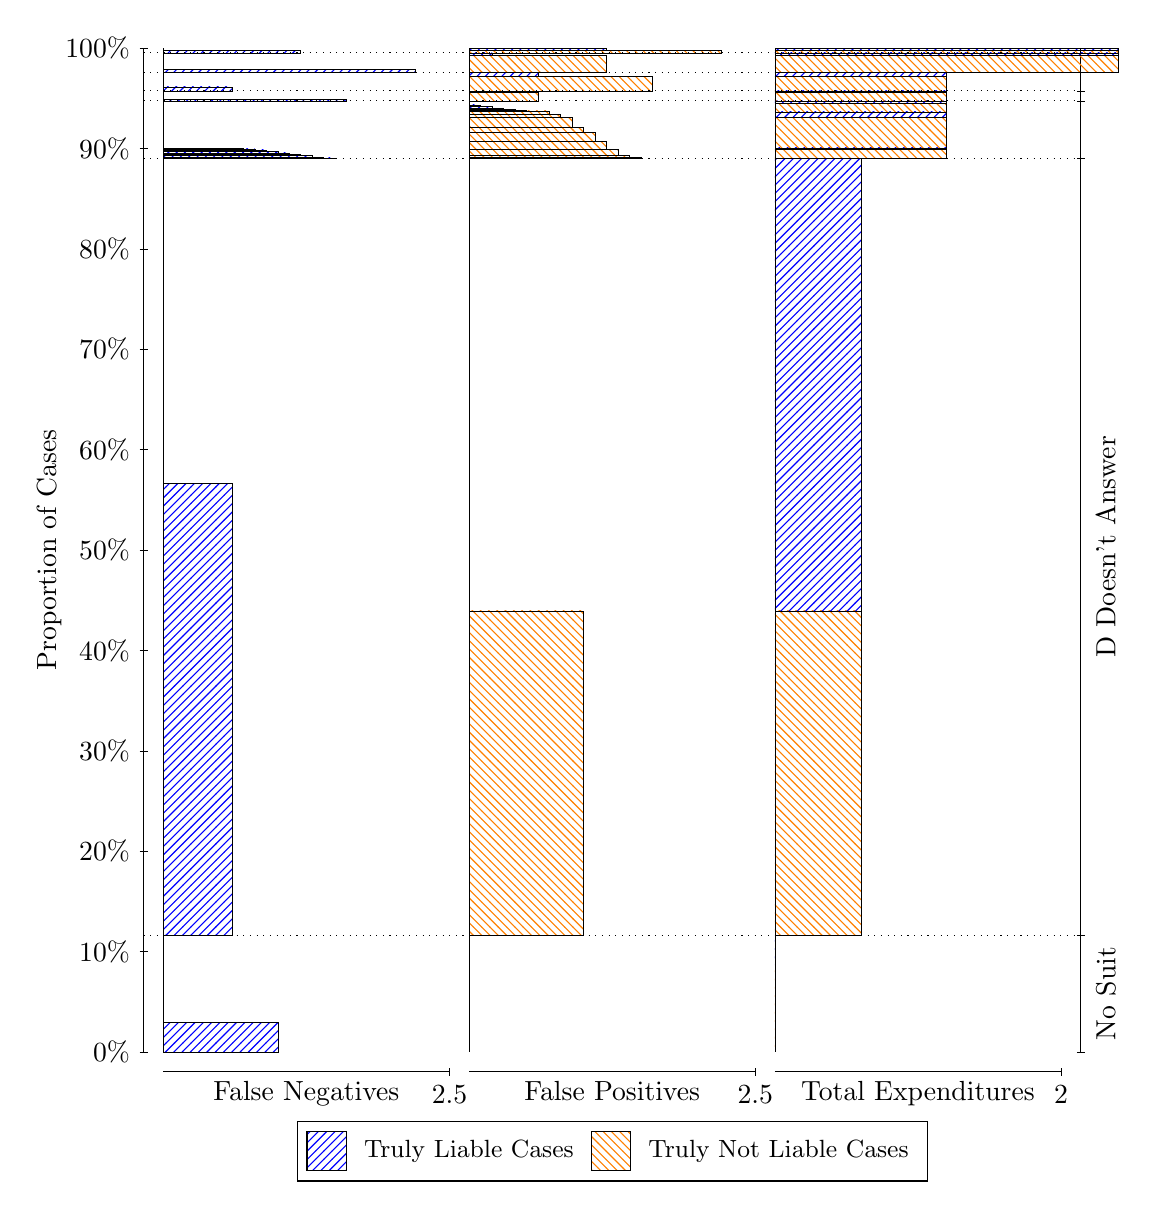
\begin{tikzpicture}
\draw[black, very thin] (1.5,1.75) -- (1.5,14.5);
\node[rotate=90, text=black, anchor=center] at (0.3, 8.125) {Proportion of Cases};
\draw[black, very thin] (1.45,1.75) -- (1.55,1.75);
\node[text=black, anchor=east] at (1.45, 1.75) {0\%};
\draw[black, very thin] (1.45,3.025) -- (1.55,3.025);
\node[text=black, anchor=east] at (1.45, 3.025) {10\%};
\draw[black, very thin] (1.45,4.3) -- (1.55,4.3);
\node[text=black, anchor=east] at (1.45, 4.3) {20\%};
\draw[black, very thin] (1.45,5.575) -- (1.55,5.575);
\node[text=black, anchor=east] at (1.45, 5.575) {30\%};
\draw[black, very thin] (1.45,6.85) -- (1.55,6.85);
\node[text=black, anchor=east] at (1.45, 6.85) {40\%};
\draw[black, very thin] (1.45,8.125) -- (1.55,8.125);
\node[text=black, anchor=east] at (1.45, 8.125) {50\%};
\draw[black, very thin] (1.45,9.4) -- (1.55,9.4);
\node[text=black, anchor=east] at (1.45, 9.4) {60\%};
\draw[black, very thin] (1.45,10.675) -- (1.55,10.675);
\node[text=black, anchor=east] at (1.45, 10.675) {70\%};
\draw[black, very thin] (1.45,11.95) -- (1.55,11.95);
\node[text=black, anchor=east] at (1.45, 11.95) {80\%};
\draw[black, very thin] (1.45,13.225) -- (1.55,13.225);
\node[text=black, anchor=east] at (1.45, 13.225) {90\%};
\draw[black, very thin] (1.45,14.5) -- (1.55,14.5);
\node[text=black, anchor=east] at (1.45, 14.5) {100\%};

\draw[black, very thin] (13.4,1.75) -- (13.4,14.5);
\draw[black, very thin] (13.35,1.75) -- (13.45,1.75);
\node[anchor=west] at (13.35, 1.75) {};
\draw[black, very thin] (13.35,3.2317) -- (13.45,3.2317);
\node[anchor=west] at (13.35, 3.2317) {};
\draw[black, very thin] (13.35,13.095) -- (13.45,13.095);
\node[anchor=west] at (13.35, 13.095) {};
\draw[black, very thin] (13.35,13.829) -- (13.45,13.829);
\node[anchor=west] at (13.35, 13.829) {};
\draw[black, very thin] (13.35,13.957) -- (13.45,13.957);
\node[anchor=west] at (13.35, 13.957) {};
\draw[black, very thin] (13.35,14.192) -- (13.45,14.192);
\node[anchor=west] at (13.35, 14.192) {};
\draw[black, very thin] (13.35,14.439) -- (13.45,14.439);
\node[anchor=west] at (13.35, 14.439) {};
\draw[black, very thin] (13.35,14.5) -- (13.45,14.5);
\node[anchor=west] at (13.35, 14.5) {};

\draw[black, very thin, pattern color=blue, pattern=north east lines] (1.75,1.75) rectangle (3.2033,2.1288);
\draw[black, very thin, pattern color=orange, pattern=north west lines] (1.75,2.1288) rectangle (1.75,3.2317);
\draw[black, very thin, pattern color=blue, pattern=north east lines] (1.75,3.2317) rectangle (2.622,8.9739);
\draw[black, very thin, pattern color=orange, pattern=north west lines] (1.75,8.9739) rectangle (1.75,13.095);
\draw[black, very thin, pattern color=blue, pattern=north east lines] (1.75,13.095) rectangle (3.93,13.106);
\draw[black, very thin, pattern color=blue, pattern=north east lines] (1.75,13.106) rectangle (3.7847,13.114);
\draw[black, very thin, pattern color=blue, pattern=north east lines] (1.75,13.114) rectangle (3.6393,13.133);
\draw[black, very thin, pattern color=blue, pattern=north east lines] (1.75,13.133) rectangle (3.494,13.147);
\draw[black, very thin, pattern color=blue, pattern=north east lines] (1.75,13.147) rectangle (3.3487,13.169);
\draw[black, very thin, pattern color=blue, pattern=north east lines] (1.75,13.169) rectangle (3.2033,13.186);
\draw[black, very thin, pattern color=blue, pattern=north east lines] (1.75,13.186) rectangle (3.058,13.207);
\draw[black, very thin, pattern color=blue, pattern=north east lines] (1.75,13.207) rectangle (2.9127,13.219);
\draw[black, very thin, pattern color=blue, pattern=north east lines] (1.75,13.219) rectangle (2.7673,13.223);
\draw[black, very thin, pattern color=orange, pattern=north west lines] (1.75,13.223) rectangle (1.75,13.829);
\draw[black, very thin, pattern color=blue, pattern=north east lines] (1.75,13.829) rectangle (4.0753,13.843);
\draw[black, very thin, pattern color=orange, pattern=north west lines] (1.75,13.843) rectangle (1.75,13.957);
\draw[black, very thin, pattern color=blue, pattern=north east lines] (1.75,13.957) rectangle (2.622,14.006);
\draw[black, very thin, pattern color=orange, pattern=north west lines] (1.75,14.006) rectangle (1.75,14.192);
\draw[black, very thin, pattern color=blue, pattern=north east lines] (1.75,14.192) rectangle (4.9473,14.224);
\draw[black, very thin, pattern color=orange, pattern=north west lines] (1.75,14.224) rectangle (1.75,14.439);
\draw[black, very thin, pattern color=blue, pattern=north east lines] (1.75,14.439) rectangle (3.494,14.468);
\draw[black, very thin, pattern color=orange, pattern=north west lines] (1.75,14.468) rectangle (1.75,14.5);
\draw[black, very thin, pattern color=orange, pattern=north west lines] (5.6333,1.75) rectangle (5.6333,2.8529);
\draw[black, very thin, pattern color=blue, pattern=north east lines] (5.6333,2.8529) rectangle (5.6333,3.2317);
\draw[black, very thin, pattern color=orange, pattern=north west lines] (5.6333,3.2317) rectangle (7.0867,7.3526);
\draw[black, very thin, pattern color=blue, pattern=north east lines] (5.6333,7.3526) rectangle (5.6333,13.095);
\draw[black, very thin, pattern color=orange, pattern=north west lines] (5.6333,13.095) rectangle (7.8133,13.108);
\draw[black, very thin, pattern color=orange, pattern=north west lines] (5.6333,13.108) rectangle (7.668,13.139);
\draw[black, very thin, pattern color=orange, pattern=north west lines] (5.6333,13.139) rectangle (7.5227,13.216);
\draw[black, very thin, pattern color=orange, pattern=north west lines] (5.6333,13.216) rectangle (7.3773,13.31);
\draw[black, very thin, pattern color=orange, pattern=north west lines] (5.6333,13.31) rectangle (7.232,13.426);
\draw[black, very thin, pattern color=orange, pattern=north west lines] (5.6333,13.426) rectangle (7.0867,13.496);
\draw[black, very thin, pattern color=orange, pattern=north west lines] (5.6333,13.496) rectangle (6.9413,13.618);
\draw[black, very thin, pattern color=orange, pattern=north west lines] (5.6333,13.618) rectangle (6.796,13.658);
\draw[black, very thin, pattern color=orange, pattern=north west lines] (5.6333,13.658) rectangle (6.6507,13.701);
\draw[black, very thin, pattern color=blue, pattern=north east lines] (5.6333,13.701) rectangle (6.36,13.704);
\draw[black, very thin, pattern color=blue, pattern=north east lines] (5.6333,13.704) rectangle (6.2147,13.717);
\draw[black, very thin, pattern color=blue, pattern=north east lines] (5.6333,13.717) rectangle (6.0693,13.738);
\draw[black, very thin, pattern color=blue, pattern=north east lines] (5.6333,13.738) rectangle (5.924,13.754);
\draw[black, very thin, pattern color=blue, pattern=north east lines] (5.6333,13.754) rectangle (5.7787,13.777);
\draw[black, very thin, pattern color=blue, pattern=north east lines] (5.6333,13.777) rectangle (5.6333,13.829);
\draw[black, very thin, pattern color=orange, pattern=north west lines] (5.6333,13.829) rectangle (6.5053,13.943);
\draw[black, very thin, pattern color=blue, pattern=north east lines] (5.6333,13.943) rectangle (5.6333,13.957);
\draw[black, very thin, pattern color=orange, pattern=north west lines] (5.6333,13.957) rectangle (7.9587,14.143);
\draw[black, very thin, pattern color=blue, pattern=north east lines] (5.6333,14.143) rectangle (6.5053,14.192);
\draw[black, very thin, pattern color=orange, pattern=north west lines] (5.6333,14.192) rectangle (7.3773,14.406);
\draw[black, very thin, pattern color=blue, pattern=north east lines] (5.6333,14.406) rectangle (5.924,14.439);
\draw[black, very thin, pattern color=orange, pattern=north west lines] (5.6333,14.439) rectangle (8.8307,14.47);
\draw[black, very thin, pattern color=blue, pattern=north east lines] (5.6333,14.47) rectangle (7.3773,14.5);
\draw[black, very thin, pattern color=orange, pattern=north west lines] (9.5167,1.75) rectangle (9.5167,2.8529);
\draw[black, very thin, pattern color=blue, pattern=north east lines] (9.5167,2.8529) rectangle (9.5167,3.2317);
\draw[black, very thin, pattern color=orange, pattern=north west lines] (9.5167,3.2317) rectangle (10.607,7.3526);
\draw[black, very thin, pattern color=blue, pattern=north east lines] (9.5167,7.3526) rectangle (10.607,13.095);
\draw[black, very thin, pattern color=orange, pattern=north west lines] (9.5167,13.095) rectangle (11.697,13.211);
\draw[black, very thin, pattern color=blue, pattern=north east lines] (9.5167,13.211) rectangle (11.697,13.233);
\draw[black, very thin, pattern color=orange, pattern=north west lines] (9.5167,13.233) rectangle (11.697,13.615);
\draw[black, very thin, pattern color=blue, pattern=north east lines] (9.5167,13.615) rectangle (11.697,13.688);
\draw[black, very thin, pattern color=orange, pattern=north west lines] (9.5167,13.688) rectangle (11.697,13.795);
\draw[black, very thin, pattern color=blue, pattern=north east lines] (9.5167,13.795) rectangle (11.697,13.829);
\draw[black, very thin, pattern color=orange, pattern=north west lines] (9.5167,13.829) rectangle (11.697,13.943);
\draw[black, very thin, pattern color=blue, pattern=north east lines] (9.5167,13.943) rectangle (11.697,13.957);
\draw[black, very thin, pattern color=orange, pattern=north west lines] (9.5167,13.957) rectangle (11.697,14.143);
\draw[black, very thin, pattern color=blue, pattern=north east lines] (9.5167,14.143) rectangle (11.697,14.192);
\draw[black, very thin, pattern color=orange, pattern=north west lines] (9.5167,14.192) rectangle (13.877,14.406);
\draw[black, very thin, pattern color=blue, pattern=north east lines] (9.5167,14.406) rectangle (13.877,14.439);
\draw[black, very thin, pattern color=orange, pattern=north west lines] (9.5167,14.439) rectangle (13.877,14.47);
\draw[black, very thin, pattern color=blue, pattern=north east lines] (9.5167,14.47) rectangle (13.877,14.5);
\draw[black, dotted] (1.5,3.2317) -- (13.4,3.2317);
\draw[black, dotted] (1.5,13.095) -- (13.4,13.095);
\draw[black, dotted] (1.5,13.829) -- (13.4,13.829);
\draw[black, dotted] (1.5,13.957) -- (13.4,13.957);
\draw[black, dotted] (1.5,14.192) -- (13.4,14.192);
\draw[black, dotted] (1.5,14.439) -- (13.4,14.439);
\draw[black, very thin] (1.75,1.5) -- (5.3833,1.5);
\node[text=black, anchor=north] at (3.5667, 1.5) {False Negatives};
\draw[black, very thin] (5.3833,1.45) -- (5.3833,1.55);
\node[text=black, anchor=north] at (5.3833, 1.45) {2.5};

\draw[black, very thin] (5.6333,1.5) -- (9.2667,1.5);
\node[text=black, anchor=north] at (7.45, 1.5) {False Positives};
\draw[black, very thin] (9.2667,1.45) -- (9.2667,1.55);
\node[text=black, anchor=north] at (9.2667, 1.45) {2.5};

\draw[black, very thin] (9.5167,1.5) -- (13.15,1.5);
\node[text=black, anchor=north] at (11.333, 1.5) {Total Expenditures};
\draw[black, very thin] (13.15,1.45) -- (13.15,1.55);
\node[text=black, anchor=north] at (13.15, 1.45) {2};

\node[text=black, centered, rotate=90] at (13.72, 2.4908) {No Suit};
\node[text=black, centered, rotate=90] at (13.72, 8.1632) {D Doesn't Answer};






\draw (7.449999999999999,1.5) node[draw=none] (baseCoordinate) {};
\begin{scope}[align=center]
        \matrix[scale=0.5, draw=black, below=0.5cm of baseCoordinate, nodes={draw}, column sep=0.1cm]{
            \node[rectangle, draw, minimum width=0.5cm, minimum height=0.5cm, pattern color=blue, pattern=north east lines] {}; &
            \node[draw=none, font=\small, text=black] (B) {Truly Liable Cases}; &
            \node[rectangle, draw, minimum width=0.5cm, minimum height=0.5cm, pattern color=orange, pattern=north west lines] {}; &
            \node[draw=none, font=\small, text=black] (B) {Truly Not Liable Cases}; \\
            };
\end{scope}

\end{tikzpicture}
\end{document}